% !TeX spellcheck = es_ES
%%%%%%%%%%%%%%%%%%%%%%%%%%%%%%%%%%%%%%%%%
% Stylish Article
% LaTeX Template
% Version 2.1 (1/10/15)
%
% This template has been downloaded from:
% http://www.LaTeXTemplates.com
%
% Original author:
% Mathias Legrand (legrand.mathias@gmail.com) 
% With extensive modifications by:
% Vel (vel@latextemplates.com)
% Final ACS by:
% Juan Barbosa
% License:
% CC BY-NC-SA 3.0 (http://creativecommons.org/licenses/by-nc-sa/3.0/)
%
%%%%%%%%%%%%%%%%%%%%%%%%%%%%%%%%%%%%%%%%%
\documentclass[fleqn,10pt]{SelfArx}
%\usepackage[superscript]{cite}
\usepackage{wrapfig}
\usepackage{multirow}
%----------------------------------------------------------------------------------------
%	ARTICLE INFORMATION
%----------------------------------------------------------------------------------------

\JournalInfo{Laboratorio de Bioquímica, 17/03/2019} % Journal information
\Archive{ }

\PaperTitle{Identificaci\'on de carbohidratos} %
%\Keywords{Keyword1 --- Keyword2 --- Keyword3} % Keywords - if you don't want any simply remove all the text between the curly brackets
%\newcommand{\keywordname}{Keywords} % Defines the keywords heading name

%----------------------------------------------------------------------------------------
%	ABSTRACT
%----------------------------------------------------------------------------------------

\Abstract{
	Carbohydrates are the main source of energy for both animals and humans. Carbohydrates can have different structures or properties, which allows the use of certain tests to identify them in broad strokes. Thanks to this, we sought to observe the particular behaviors of different types of carbohydrates in the face of various characteristic identification reactions. In addition, we sought to identify the nature of an unknown carbohydrate by means of characteristic identification reactions. To achieve this, three standard standards were used: maltose, sucrose and glucose, and a test sample. These samples were tested with the Molisch reaction, the Barfoed test, the Fehling test, the Seliwanoff test and the Osazone test. As a result, it was obtained that the identity of the unkown sugar is either xylose or arabinose, two carbohidrates whose behavior in all of the tested reactions is the same.
}

%----------------------------------------------------------------------------------------

\begin{document}

\flushbottom % Makes all text pages the same height

\maketitle % Print the title and abstract box
%\tableofcontents % Print the contents section

\thispagestyle{empty} % Removes page numbering from the first page



%----------------------------------------------------------------------------------------
%	ARTICLE CONTENTS
%----------------------------------------------------------------------------------------

\section*{Introducci\'on} % The \section*{} command stops section numbering
%------------------------------------------------
	En la naturaleza existen una infinidad de compuestos, los cuales han sido clasificados en inorgánicos y orgánicos \cite{ebbing2010quimica}. Dentro de la clasificación de los compuestos orgánicos, el carbono es el elemento principal. Con el carbono y otros pocos elementos, se puede formar macromoléculas biológicas, en otras palabras, polímeros de alto peso molecular formados a partir de precursores simples, comparados con la estructura final. Entre estas moléculas se encuentran las proteínas, los carbohidratos, los lípidos y los ácidos nucleicos \cite{blanco2017gustavo, nelson2008lehninger}.
	
	Centrándonos más, los carbohidratos son uno de los principales tipos de nutrientes. Son la principal fuente de energía para el cuerpo, tanto en humanos como en los animales \cite{martin2001bioquimica}. Este tipo de compuestos se descomponen a carbohidratos más pequeños, como la glucosa. Después, el cuerpo metaboliza la glucosa, produciendo Piruvato, NADH, H$^+$, agua y ATP \cite{nelson2008lehninger}, siendo el ATP energía para las células, tejidos y órganos. Por otro lado, no todos los carbohidratos que entran al cuerpo son procesados, parte de estos se guarda en el hígado y músculos para cuando se necesiten.
	
	Continuando, los carbohidratos se clasifican en simples o complejos dependiendo de su estructura química. Entre los carbohidratos simples se tiene el azúcar que se encuentra naturalmente en productos, tales como frutas, vegetales, leche y derivados de la leche. Además, dentro de los carbohidratos simples se incluyen azúcares añadidos durante el procesamiento y refinación de ciertos alimento \cite{maite}. Entre los carbohidratos complejos se tienen los panes y cereales integrales, vegetales ricos en almidón y legumbres \cite{maite}.
	
	Por otro lado, los carbohidratos también cumplen una función estructural fundamental en los organismos. Polisacáridos como el peptidoglicano por ejemplo, es el componente principal de las paredes celulares de bacterias y plantas, además de jugar un papel importante en la comunicación celular.
	
	En particular para las muestras analizadas en el presente documento se tiene lo siguiente:
	\begin{itemize}
		\item \textbf{Fructuosa} Es un importante azúcar estructural de las plantas, forma parte de la sacarosa y es un intermediario de la glucólisis, por lo que es un monosacárido muy abundante en el medio celular y constituye una de las fuentes principales de energía en las células por su disponibilidad y capacidad hidrolizable.
		
		\item \textbf{Glucosa} Es uno de los carbohidratos mas abundantes en la naturaleza y constituye la fuente principal de energía en los organismos vivos, en forma de energía metabólica. Además, esta tambien cumple un rol estructural en la celulosa, la cual es un homopolisacárido de glucosa y la biomolécula orgánica más abundante, puesto que conforma la mayor parte de la biomasa terrestre.
		
		\item \textbf{Lactosa} Esta presente en lácteos y algunos vegetales y constituye la fuente de energía fundamental en mamíferos durante el periodo de lactancia, por lo que juega un papel fundamental en el desarrollo de estos organismos.
		
		\item \textbf{Maltosa} Es un dímero de glucosa que esta presente en plantas en forma de almidón y animales en forma de glucógeno y constituye a su vez la principal reserva energética, siendo capaz de almacenar grandes cantidades de energía por medio de enlaces fácilmente aprovechables por las células, manteniendo a su vez una forma óptima de plegamiento en su estructura.
		
		\item \textbf{Sacarosa} Esta presente en los frutos, semillas, raíces y en la miel y es uno de los productos de la fotosíntesis y constituye una fuente de energía en los organismos. Además, es uno de los azúcares mas comunes y constituye el “azúcar de mesa“, por lo que es ampliamente utilizado y producido por la industria alimenticia.
	\end{itemize}
	
	En cuanto identificación, existen diferentes pruebas las cuales dan indicio de que tipo de hidrocarburos se tiene. Por ejemplo, la prueba de Benedict es una prueba en la cual se emplea el reactivo de Benedict para identificar azucares reductoras \cite{raymond2013general}, azúcares que poseen su grupo carbonilo intacto \cite{nelson2008lehninger}. Otra prueba que se tiene es la de Molisch, en la cual se tiñe cualquier carbohidrato presente en una disolución \cite{harisha2005introduction}. Tambien se tiene la prueba de Barfoed, en la cual se detecta monosacáridos, mediante la reduccion del cobre (II) a cobre (I)  \cite{barfoed1873ueber}. Otro ejemplo es la oxidación de oxidación de Fehling, la cual es una prueba análoga a la prueba de Benedit \cite{bonner1976quimica}. Otra posible prueba es la prueba de Seliwanoff, la cual permite distinguir aldosas y cetosas, azucares que contienen un grupo aldehído o cetona, respectivamente; Por ultimo se tiene la prueba de Osazone, la cual permite para identificar monosacáridos.
	
	En base a lo anterior, en esta ocasión se buscó observar los comportamientos particulares de distintos tipos de carbohidratos frente a diversas reacciones características de identificación. Para lograr esto se empleó estándares: maltosa, sacarosa y glucosa. Además, se buscó identificar la naturaleza de un carbohidrato desconocido por medio de las reacciones características de identificación, tales como la reaccion de Molisch, la prueba de Barfoed, la prueba de Fehling, prueba de Seliwanoff y la prueba de Osazone.
	\begin{table*}[h]
		\centering
		\caption{Resultados esperados para las muestras}
		\label{tb}
		\begin{tabular}{c|ccccp{1.5cm}}
			\hline
			\textbf{Muestra} & \textbf{Molisch} & \textbf{Benedict} & \textbf{Fehling} & \textbf{Seliwanoff} & \textbf{Osazone} \\
			\hline
			\textbf{Maltosa} & + & N.A. & + & - & Círculos de agujas \\
			\textbf{Glucosa} & + & N.A. & + & + & Agujas \\
			\textbf{Sacarosa} & + & N.A. & - & + & - \\
			\hline
			\textbf{Xilosa} & + & + & + & - & Agujas \\
			\textbf{Lactosa} & + & + & - & - & Círculos de agujas \\
			\textbf{Fructosa} & + & + & - & + & Agujas \\
			\textbf{Arabinosa} & + & + & + & - & Agujas \\
			\hline
		\end{tabular}
	\end{table*}
	
\section{Secci\'on experimental}
	\subsection{Materiales y reactivos}
	En cuanto a los materiales empleados se tiene: balón aforado de 10 mL, tubos de ensayo, pipeta graduada 5 mL, gotero de vidrio, beaker 400 mL, plancha de calentamiento y microscopio. En cuanto a reactivos, se empleó: solución estandar al 5 \% p/v de glucosa, sacarosa, maltosa y muestra problema, solución de $\alpha$-Naftol al 10 \% en etanol absoluto, ácido sulfúrico concentrado, reactivo de Barfoed (0,65 g de acetato de cobre en 0,1 mL de ácido acético glacial, llevado a 10 mL con agua destilada), solucion de sulfato de cobre (II) (0,34 g de sulfato de hierro (II) anhidro en 10 mL de agua destilada), solución de hidróxido de sodio al 10 \%, soluci\'on de tartrato de sodio y potasio al 35 \% (preparada con la solución de hidróxido de sodio), solución de ácido clorhídrico al 20 \%, reactivo de Seliwanoff (5 mg de resorcinol disueltos en ácido clorhídrico al 20 \%), reactivo de Benedict y mezcla de Osazone (mezcla 1:2 de fenilhidrazina y acetato de sodio). Los materiales y reactivos fueron provistos por el laboratorio. Las soluciones fueron preparadas el mismo día de la practica. La muestra problema fue provista por la profesora.
	
	\subsection{Reacción de Molisch}
	Se tomaron 4 tubos de ensayo y se rotularon del 1 al 4. Al tubo uno se agreg\'o 1 mL de la solución de maltosa, al dos 1 mL de la solución de glucosa, al tres 1 mL de la solución de sacarosa y al cuatro 1 mL de la solución de la muestra problema. Seguidamente se añadió 5 gotas de la solucion de $\alpha$-Naftol a cada tubo. Después, se agreg\'o 2 mL de \'acido sulfúrico concentrado, por las paredes y sin revolver, a cada tubo.
	
	\subsection{Oxidación de Fehling}
	Se rotulo cuadros tubos de ensayo, del 1 al 4. A cada tubo se añadió 1 mL de la solucion de sulfato de cobre (II) y 1 mL de la solucion básica de tartrato de sodio y potasio. Seguidamente los tubos se calentaron a ebullición por 1 min. Después, al tubo uno se agrego 1 mL de la solución de maltosa, al dos 1 mL de la solución de glucosa, al tres 1 mL de la solución de sacarosa y al cuatro 1 mL de la solución de la muestra problema.
	
	\subsection{Prueba de Seliwanoff}
	Se tomaron 4 tubos de ensayo y se rotularon del 1 al 4. Al tubo uno se agregó 1 mL de la solución de maltosa, al dos 1 mL de la solución de glucosa, al tres 1 mL de la solución de sacarosa y al cuatro 1 mL de la solución de la muestra problema. Después se agrego 5 gotas del reactivo de Seliwanoff a cada tubo. Los tubos se agitaron y seguidamente se colocaron en baño maría a ebullición por 1 min.
	
	\subsection{Prueba de Osazone} 
	Se tomaron 4 tubos de ensayo y se rotularon del 1 al 4. Al tubo uno se agregó 1 mL de la solución de maltosa, al dos 1 mL de la solución de glucosa, al tres 1 mL de la solución de sacarosa y al cuatro 1 mL de la solución de la muestra problema. A continuación, se agregaron 0,2 g de la mezcla de Osazone y dos gotas de \'acido acético a cada tubo. Después, los tubos se agitaron y seguidamente se colocaron en baño maría a ebullición hasta que se formaron cristales. Finalmente, los cristales obtenidos fueron observados al microscopio.
	
	\subsection{Prueba de Benedict} Se tom\'o 1 mL de la solución de muestra problema y se añadió 1 mL de reactivo de Benedict.
	
\section{Resultados y Discusi\'on}
	Los resultados obtenidos en las pruebas bioqu\'imicas realizadas se muestra en la \autoref{tb}. En la primera secci\'on se describen las observaciones para los est\'andares usados en la pr\'actica, mientras que en la segunda se presentan lo que se deber\'ia observar para cada una de las muestras problema.
	
	\subsection{Molisch}
		La reacci\'on de Molisch es de particular importancia, dado que permite determinar la presencia de carbohidratos en la muestra \cite{blanco2017gustavo}. Si bien no es del todo selectiva a \'estos, pues da positiva para glicoprote\'inas y \'acidos nucl\'eicos, en el caso de las muestras trabajadas, considerando su pureza, los resultados muestran que todas las muestras trabajadas constituyen carbohidratos.
		\begin{scheme}[h]
			\centering
			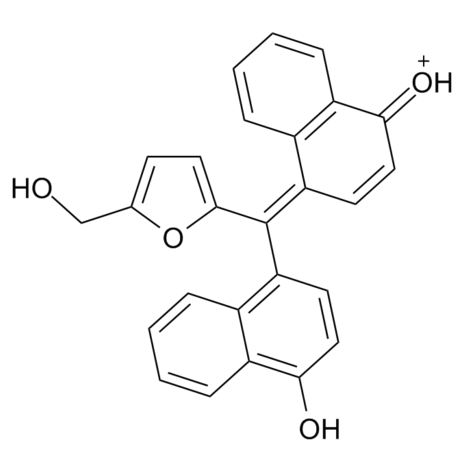
\includegraphics[width = 0.5\linewidth]{molisch}
			\caption{Complejo violeta en la reacci\'on de Molisch, para una hexoxa.}
			\label{molisch}
		\end{scheme}
	
		Se considera que un resultado positivo para la prueba de Molisch es la formaci\'on de un anillo violeta en la interfase entre el \'acido sulf\'urico y el carbohidrato. El anillo violeta tiene su origen en la formaci\'on de un complejo org\'anico altamente arom\'atico, el cual se observa en el \autoref{molisch}. Este complejo est\'a formado por un hidroximetil furfural, para el caso de carbohidratos de 6 carbonos, o furfural, para pentosas y dos derivados fen\'olicos como el $\alpha$-naftol. Los furfurales se forman independientemente del n\'umero de unidades que conformen el polisacarido o monosac\'arido, dado que la presencia del \'acido sulf\'urico, el cual, debido a su car\'acter de \'acido mineral, es cap\'az de hidrolizar polisacaridos a monosac\'aridos \cite{harisha2005introduction}.	
		
	\subsection{Barfoed}
		En el caso del reactivo de Barfoed, si bien, no se obtuvo ning\'un resultado positivo para las muestras, se debe tener en cuenta que este se comporta como un ácido débil el cual puede sufrir un proceso de reducción por acción de monosacáridos. El resultado de la prueba es positivo cuando se presenta una reacción de color rojizo, que se produce por la formación de oxido de cobre.
	
	\subsection{Benedict}
		La prueba de Benedict permite determinar la existencia de azucares reductores en el medio. Esto se debe a que, en medio fuertemente alcalino, el ion \ce{Cu^{+2}} puede ser reducido a \ce{Cu^{+1}} bajo la acci\'on del grupo aldeh\'ido de un azúcar. La reacción produce un cambio en el color desde azul, hasta, anaranjado y rojo, dependiendo de la cantidad de sustancias reductoras en la muestra. En particular, se debe destacar que la prueba se realiz\'o \'unicamente para la muestra problema, obteniendo una coloraci\'on naranja, positiva para azúcar reductor.
		
	\begin{figure*}[h]
		\centering
		\begin{tabular}{ccc}
			\fbox{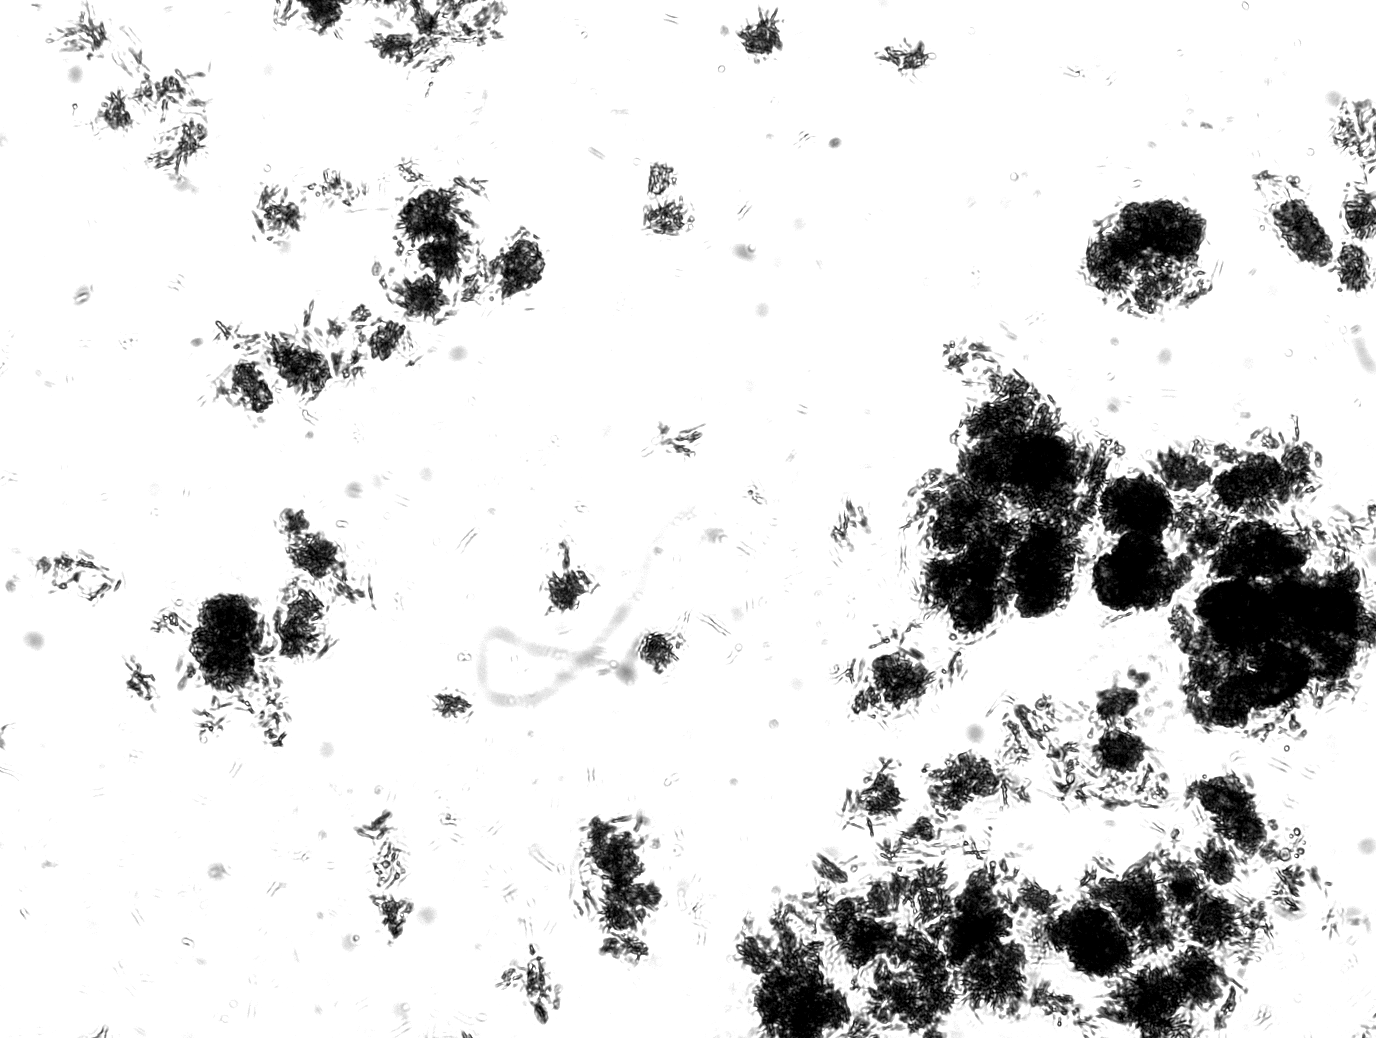
\includegraphics[width=0.3\linewidth]{Maltosa}} & 
			\fbox{
\includegraphics[width=0.3\linewidth]{Glucosa}} & 
			\fbox{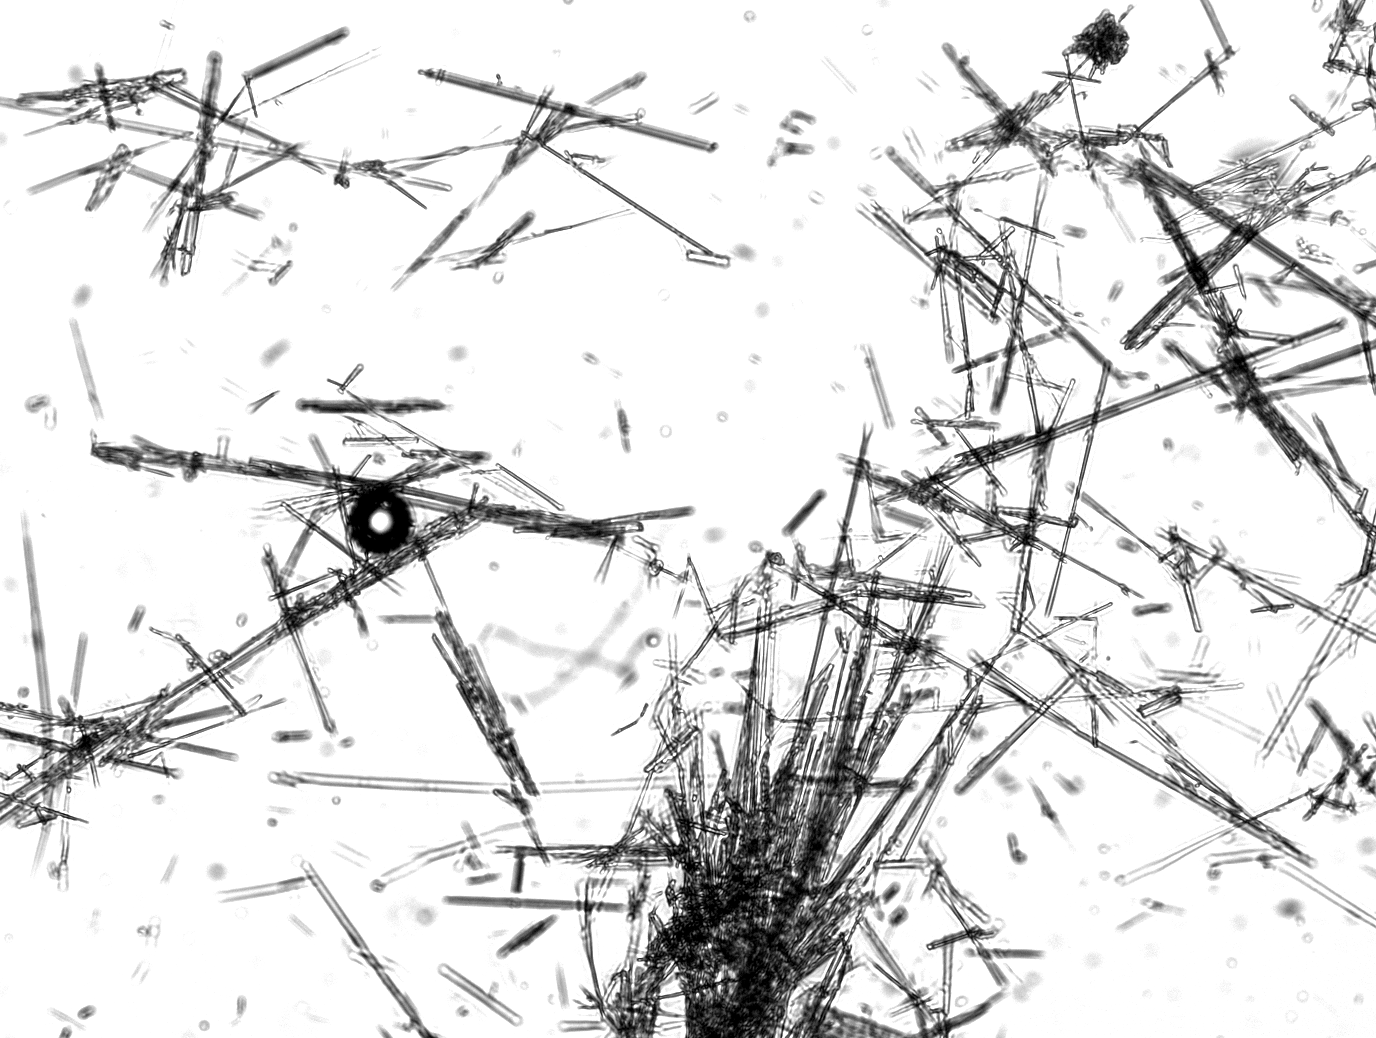
\includegraphics[width=0.3\linewidth]{Problema}}
		\end{tabular}
		\caption{De izquierda a derecha: maltosa, glucosa y la muestra problema. Im\'agenes tomadas con una camara CCD Olympus a una magnificaci\'on de 20 x.}
		\label{fig}
	\end{figure*}
			
	\subsection{Fehling}
		La prueba de Fehling, al igual que la de Benedict y Barfoed, tambi\'en permite determinar la presencia de carbohidratos reductores. Si bien el mecanismo es an\'alogo al de Benedict, en donde la coloraci\'on observada se debe a la reducci\'on del ion cobre (II) a cobre (I), esta reducci\'on sucede \'unicamente a trav\'es de \'acidos carbox\'ilicos, los cuales se obtienen a partir de la oxidaci\'on del grupo aldeh\'ido de los carbohidratos. En muchos casos, la reacci\'on permite distinguir entre aldosas y cetosas reductoras, dado que las cetonas no pueden oxidarse a \'acidos carbox\'ilicos, a menos que sean $\alpha$-hidroxicetonas. Es por esta raz\'on que en las muestras problema, la fructuosa, a pesar de ser una cetona da positivo, pues es posible que debido al medio alcalino, se tautomerice la estructura, produciendo un alcohol el cual posteriormente se oxida a \'acido. De esta forma, y a partir de los resultados obtenidos en el laboratorio, se descarta la presencia de lactosa en la muestra problema.
		
		Por otro lado, la maltosa, si bien no es un monosac\'arido, da positivo a la reacci\'on dado que \'esta procede sobre la cadena abierta, la cual presenta el aldeh\'ido propio de la glucosa \cite{ouellette2015principles}.
	
	\subsection{Seliwanoff}
		El principio de funcionamiento de la prueba de Seliwanoff consiste en que: las cetosas, como la fructuosa, en presencia de calor y en un medio ácido, forman un derivado de furfural el cual se combina con el resorcinol presente en la soluci\'on formando un compuesto de color rojo. Esta prueba es espec\'ifica para cetosas, raz\'on por la cual se esperar\'ia que los \'unicos resultados positivos fueran para la fructuosa y la sacarosa (el cual contiene fructuosa), sin embargo, como se observa en la \autoref{tb}, tambi\'en se observ\'o un resultado positivo para la glucosa, la cual corresponde con una aldosa. 
		
		A nivel experimental, se observ\'o un color lig\'eramente amarillo para la muestra problema, lo cual bien podr\'ia asociarse a la presencia de cetosas en la misma. Sin embargo, al considerar los tiempos de la reacci\'on, la coloraci\'on tuvo lugar en tiempos an\'alogos a los observados para el falso positivo de la glucosa, los cuales fueron considerablemente superiores a los de la sacarosa. A partir de esto se considera que la muestra tuvo, en realidad un resultado negativo para la prueba.
		
	\subsection{Osazone}
		Los resultados de la prueba de Osazone se muestran en la \autoref{fig}, en ella se pueden observar los c\'irculos de agujas caracter\'isticos para disac\'aridos reductores como la maltosa y la lactosa, y las agujas propias de los monosac\'aridos reductores. De la \autoref{tb}, la sacarosa no form\'o cristales dado que es la \'unica que no constituye un azúcar reductor.
		
		La reacci\'on tiene lugar cuando un az\'ucar reductor reacciona con dos equivalentes de fenilhidrazina, las cuales sustituyen el grupo carbonilo y el OH del carbono $\alpha$, en la cadena abierta, como se observa en el \autoref{osazone}.
		\begin{scheme}[h]
			\centering
			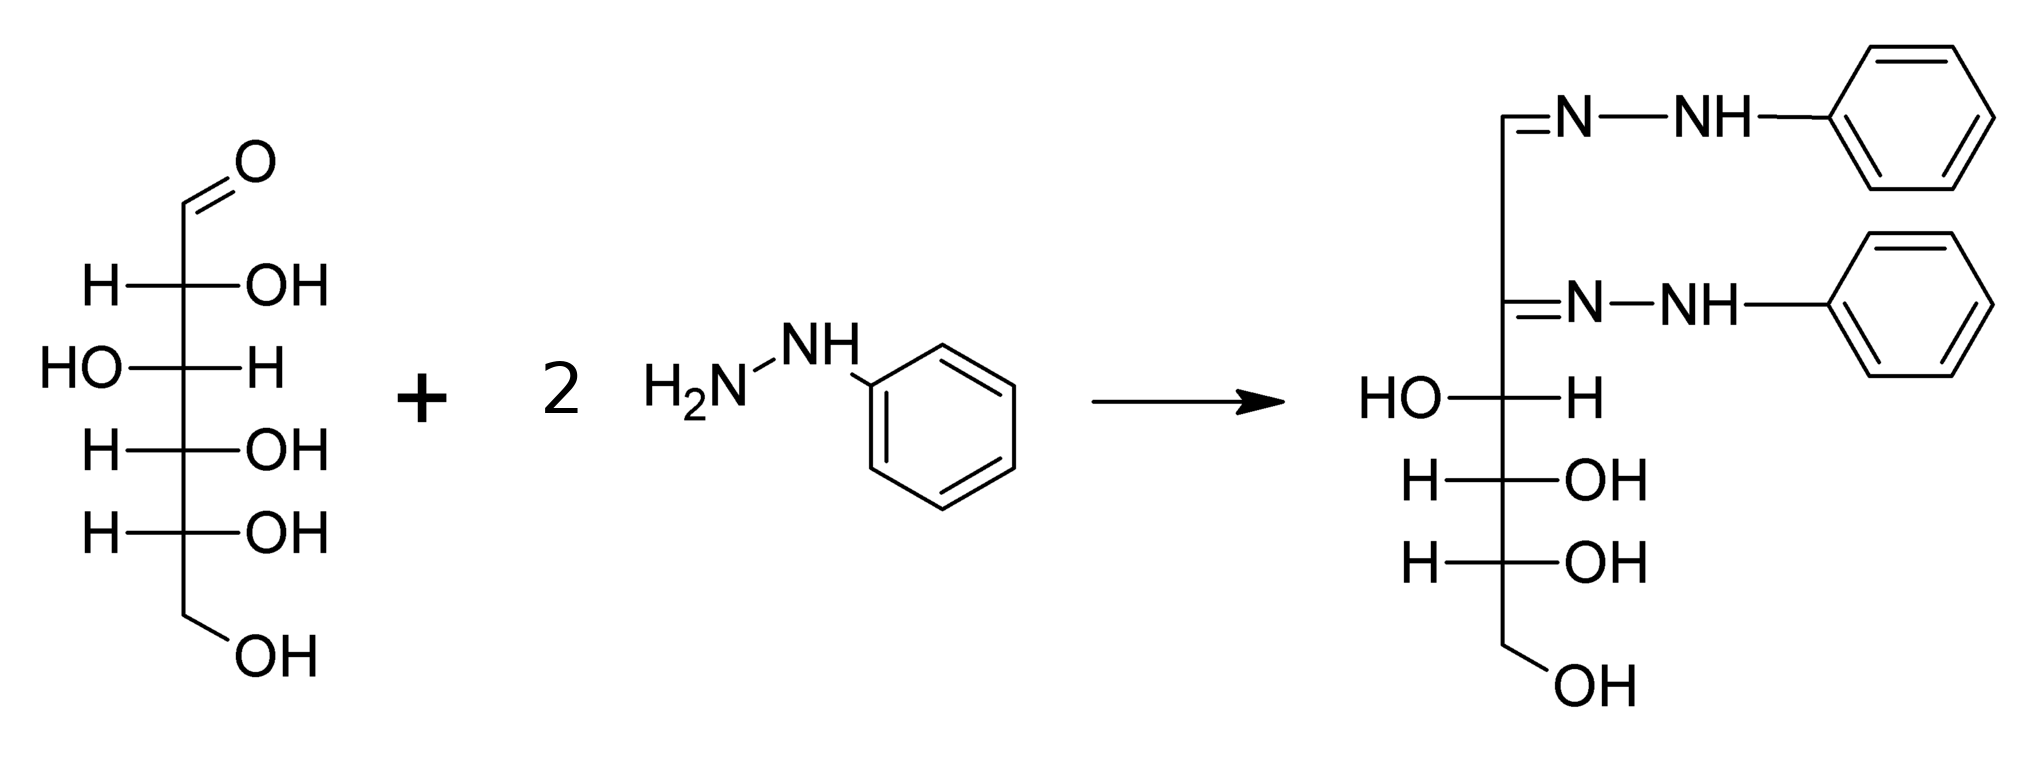
\includegraphics[width=\linewidth]{osazone}
			\caption{Formaci\'on de la osazona de la glucosa.}
			\label{osazone}
		\end{scheme}
	
		Los resultados de la prueba de Osazone, confirman los resultados obtenidos hasta el momento, los cuales apuntan a que la muestra problema es xilosa, o arabinosa, dos aldopentosas, que no son distinguibles a partir de las pruebas bioqu\'imicas realizadas en el laboratorio. Sobre esta \'ultima vale la pena mencionar que esta se encuentra presente en algunas plantas como componente de las paredes celulares y bacterianas como es el caso de los bacilos de la tuberculosis, por lo que puede jugar un papel importante en la tipificación de estos organismos y, asi mismo, el control de enfermedades emergentes en la población que pueden constituir un problema de salud pública. Adicionalmente, este carbohidrato se encuentra presente también en la goma arabiga, la cuál es ampliamente usada en la industria de alimentos como agente gelificante.
		
	
\section{Conclusiones}
	Usando pruebas bioqu\'imicos, fue posible establecer la naturaleza de az\'ucar reductor de la muestra problema. Adicionalmente, la prueba de Fehling en conjunto con la reacci\'on de Seliwanoff permit\'io determinar la presencia del grupo aldeh\'ido en la muestra. La formaci\'on de cristales tipo aguja, en la prueba de Osazone, confirma la presencia de un az\'ucar monosac\'arido, limitando la identidad del mismo a xilosa y arabinosa, dos aldosas que no puden ser distinguidas por los m\'etodos aqu\'i reportados.
	
	Cada uno de las reacciones fue explicada, junto con los resultados obtenidos para los est\'andares y las posibles identidades de las muestras problema. Todos los resultados observados fueron consistentes, salvo por la glucosa en la reacci\'on de Seliwanoff.
	
	Por \'ultimo, dada la importancia biol\'ogica de los carbohidratos, se hizo una breve introducci\'on sobre la presencia de los az\'ucares trabajados en organismos vivos, junto con sus funciones principales en ellos.
%----------------------------------------------------------------------------------------
%	REFERENCE LIST
%----------------------------------------------------------------------------------------
\phantomsection
\bibliography{informe}
\bibliographystyle{unsrt}

%----------------------------------------------------------------------------------------
%\newpage
%\onecolumn
%\section{Informaci\'on suplementaria}\label{sec: complementaria}
\end{document}